\documentclass[10pt]{article}
\usepackage[polish]{babel}
\usepackage[utf8]{inputenc}
\usepackage[T1]{fontenc}
\usepackage{graphicx}
\usepackage[export]{adjustbox}
\graphicspath{ {./images/} }
\usepackage{amsmath}
\usepackage{amsfonts}
\usepackage{amssymb}
\usepackage[version=4]{mhchem}
\usepackage{stmaryrd}

\title{LICEUM }

\author{GIMNAZJUM}
\date{}


\begin{document}
\maketitle
Zestaw 6.\\

\includegraphics[max width=\textwidth, center]{2024_11_21_da23055957b186aca865g-1}

MATEMATYKI



\begin{enumerate}
  \item Udowodnij, że jeżeli pewną liczbę można przedstawić jaką różnicę kwadratów dwóch liczb naturalnych to również jej trzykrotność można przedstawić jako różnicę kwadratów dwóch liczb naturalnych.
  \item Dany jest trójkąt prostokątny, w którym kąt przy wierzchołku \(C\) jest prosty oraz \(|A C| \neq|B C|\). Punkty \(P\) i \(Q\) są takie, że czworokąt \(A P B Q\) jest kwadratem. Udowodnij, że proste \(C P\) i \(C Q\) są prostopadłe.
  \item Liczby rzeczywiste \(a, b, c, d\) spełniają równości\\
\((a+b)(c+d)=(a+c)(b+d)=(a+d)(b+c)\)\\
Udowodnij, że co najmniej trzy z liczb \(a, b, c, d\) są równe.
\end{enumerate}

\begin{enumerate}
  \item Czworokąt \(A B C D\) jest wpisany w okrąg. Proste \(A B\) i \(C D\) przecinają się w punkcie \(E\), a proste \(A D\) i \(B C\) przecinają się w punkcie \(F\). Udowodnij, że jeśli \(B E=D F\), to \(C E=C F\).\\
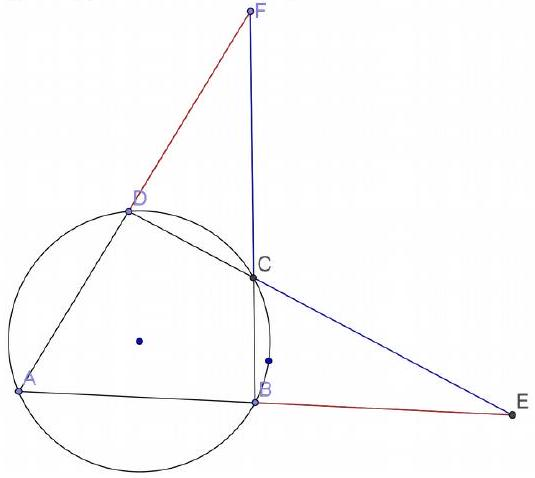
\includegraphics[max width=\textwidth, center]{2024_11_21_da23055957b186aca865g-1(1)}
  \item Na brzegu kwadratu o boku \(n\) ( \(n \geq 2\) jest liczbą naturalną) wyróżniono \(2 n\) punktów różnych od wierzchołków, które dzielą każdy z boków na odcinki o całkowitych długościach. Udowodnij, że pewne cztery wyróżnione punkty są wierzchołkami równoległoboku, którego środek pokrywa się z środkiem kwadratu.\\
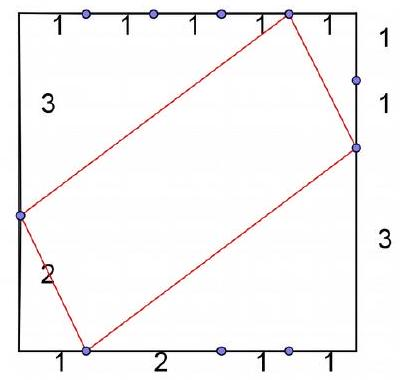
\includegraphics[max width=\textwidth, center]{2024_11_21_da23055957b186aca865g-1(2)}
  \item Dane są dwa okręgi współśrodkowe - mniejszy o promieniu \(r\) i większy o promieniu \(R\). Przez wybrany punkt mniejszego okręgu poprowadzono parę prostych prostopadłych. Oblicz sumę kwadratów długości odcinków wyciętych z tych prostych przez większy okrąg.
\end{enumerate}

Rozwiq̨zania należy oddać do piqtku 6 marca do godziny 12.30 koordynatorowi konkursu panu Jarosławowi Szczepaniakowi lub swojemu nauczycielowi matematyki.

Na stronie internetowej szkoły w zakładce „Konkursy i olimpiady" można znaleźć wyniki dotychczasowych rund i rozwiązania zadań.


\end{document}